\documentclass[]{article}
\usepackage{lmodern}
\usepackage{amssymb,amsmath}
\usepackage{ifxetex,ifluatex}
\usepackage{fixltx2e} % provides \textsubscript
\ifnum 0\ifxetex 1\fi\ifluatex 1\fi=0 % if pdftex
  \usepackage[T1]{fontenc}
  \usepackage[utf8]{inputenc}
\else % if luatex or xelatex
  \ifxetex
    \usepackage{mathspec}
  \else
    \usepackage{fontspec}
  \fi
  \defaultfontfeatures{Ligatures=TeX,Scale=MatchLowercase}
\fi
% use upquote if available, for straight quotes in verbatim environments
\IfFileExists{upquote.sty}{\usepackage{upquote}}{}
% use microtype if available
\IfFileExists{microtype.sty}{%
\usepackage{microtype}
\UseMicrotypeSet[protrusion]{basicmath} % disable protrusion for tt fonts
}{}
\usepackage[margin=1in]{geometry}
\usepackage{hyperref}
\hypersetup{unicode=true,
            pdftitle={DATA 605 - Assignment 10},
            pdfauthor={Joshua Sturm},
            pdfborder={0 0 0},
            breaklinks=true}
\urlstyle{same}  % don't use monospace font for urls
\usepackage{graphicx,grffile}
\makeatletter
\def\maxwidth{\ifdim\Gin@nat@width>\linewidth\linewidth\else\Gin@nat@width\fi}
\def\maxheight{\ifdim\Gin@nat@height>\textheight\textheight\else\Gin@nat@height\fi}
\makeatother
% Scale images if necessary, so that they will not overflow the page
% margins by default, and it is still possible to overwrite the defaults
% using explicit options in \includegraphics[width, height, ...]{}
\setkeys{Gin}{width=\maxwidth,height=\maxheight,keepaspectratio}
\IfFileExists{parskip.sty}{%
\usepackage{parskip}
}{% else
\setlength{\parindent}{0pt}
\setlength{\parskip}{6pt plus 2pt minus 1pt}
}
\setlength{\emergencystretch}{3em}  % prevent overfull lines
\providecommand{\tightlist}{%
  \setlength{\itemsep}{0pt}\setlength{\parskip}{0pt}}
\setcounter{secnumdepth}{0}
% Redefines (sub)paragraphs to behave more like sections
\ifx\paragraph\undefined\else
\let\oldparagraph\paragraph
\renewcommand{\paragraph}[1]{\oldparagraph{#1}\mbox{}}
\fi
\ifx\subparagraph\undefined\else
\let\oldsubparagraph\subparagraph
\renewcommand{\subparagraph}[1]{\oldsubparagraph{#1}\mbox{}}
\fi

%%% Use protect on footnotes to avoid problems with footnotes in titles
\let\rmarkdownfootnote\footnote%
\def\footnote{\protect\rmarkdownfootnote}

%%% Change title format to be more compact
\usepackage{titling}

% Create subtitle command for use in maketitle
\newcommand{\subtitle}[1]{
  \posttitle{
    \begin{center}\large#1\end{center}
    }
}

\setlength{\droptitle}{-2em}
  \title{DATA 605 - Assignment 10}
  \pretitle{\vspace{\droptitle}\centering\huge}
  \posttitle{\par}
  \author{Joshua Sturm}
  \preauthor{\centering\large\emph}
  \postauthor{\par}
  \predate{\centering\large\emph}
  \postdate{\par}
  \date{April 15, 2018}


\begin{document}
\maketitle

\section{Question 1}\label{question-1}

Smith is in jail and has 1 dollar; he can get out on bail if he has 8
dollars. A guard agrees to make a series of bets with him. If Smith bets
A dollars, he wins A dollars with probability .4 and loses A dollars
with probability .6. Find the probability that he wins 8 dollars before
losing all of his money if

\subsection{(a) he bets 1 dollar each time (timid
strategy).}\label{a-he-bets-1-dollar-each-time-timid-strategy.}

\subsection{(b) he bets, each time, as much as possible but not more
than necessary to bring his fortune up to 8 dollars (bold
strategy).}\label{b-he-bets-each-time-as-much-as-possible-but-not-more-than-necessary-to-bring-his-fortune-up-to-8-dollars-bold-strategy.}

\subsection{(c) Which strategy gives Smith the better chance of getting
out of
jail?}\label{c-which-strategy-gives-smith-the-better-chance-of-getting-out-of-jail}

\section{Solutions}\label{solutions}

This is known as the Gambler's Ruin problem.

We are given:

Initial stake \(z = k = 1\).

\(M = 8\)

\(P = 0.4\)

\(q = 0.6\)

\(q_z = \frac{(\frac{q}{p})^z - 1}{(\frac{q}{p})^M - 1}\)

\subsection{(a)}\label{a}

\(q_z = \frac{(\frac{0.6}{0.4})^1 - 1}{(\frac{0.6}{0.4})^8 - 1} =\)
0.0203013.

There is a \textasciitilde{}2\% probability Smith will win using this
strategy.

\subsection{(b)}\label{b}

The quickest strategy is if he bets everything each time. That is,
beginning from state \(z = k = 1\), he can move fall to 0 with
\(q = 0.6\), or rise to 2 with \(p = 0.4\). Similarly, suppose he moved
to 2, he bets everything, and can fall to 0 with \(q = 0.6\), or rise to
4 with \(p = 0.4\).

\begin{figure}
\centering
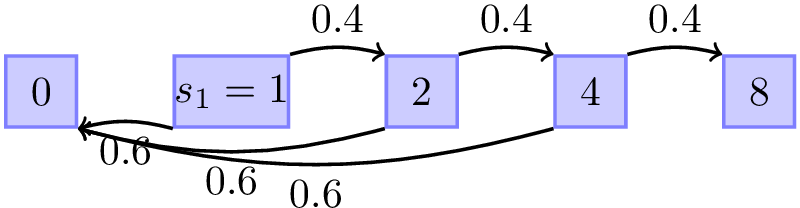
\includegraphics{markov.png}
\caption{}
\end{figure}

Using the formula \(q_k = p\cdot q_{k+1} + q\cdot q{k-1}\):

\(q_0 = 0\)

\(q_1 = (0.4)q_2 + (0.6)q_0\)

\(q_2 = (0.4)q_4 + (0.6)q_0\)

\(q_4 = (0.4)q_8 + (0.6)q_0\)

\(q_8 = 1\)

\((0.4)^3 =\) 0.064.

\section{References}\label{references}

\begin{itemize}
\tightlist
\item
  \url{http://people.math.umass.edu/~lr7q/ps_files/teaching/math456/Week4.pdf}
\end{itemize}


\end{document}
